% GNUPLOT: LaTeX picture with Postscript
\begingroup
  \makeatletter
  \providecommand\color[2][]{%
    \GenericError{(gnuplot) \space\space\space\@spaces}{%
      Package color not loaded in conjunction with
      terminal option `colourtext'%
    }{See the gnuplot documentation for explanation.%
    }{Either use 'blacktext' in gnuplot or load the package
      color.sty in LaTeX.}%
    \renewcommand\color[2][]{}%
  }%
  \providecommand\includegraphics[2][]{%
    \GenericError{(gnuplot) \space\space\space\@spaces}{%
      Package graphicx or graphics not loaded%
    }{See the gnuplot documentation for explanation.%
    }{The gnuplot epslatex terminal needs graphicx.sty or graphics.sty.}%
    \renewcommand\includegraphics[2][]{}%
  }%
  \providecommand\rotatebox[2]{#2}%
  \@ifundefined{ifGPcolor}{%
    \newif\ifGPcolor
    \GPcolorfalse
  }{}%
  \@ifundefined{ifGPblacktext}{%
    \newif\ifGPblacktext
    \GPblacktexttrue
  }{}%
  % define a \g@addto@macro without @ in the name:
  \let\gplgaddtomacro\g@addto@macro
  % define empty templates for all commands taking text:
  \gdef\gplbacktext{}%
  \gdef\gplfronttext{}%
  \makeatother
  \ifGPblacktext
    % no textcolor at all
    \def\colorrgb#1{}%
    \def\colorgray#1{}%
  \else
    % gray or color?
    \ifGPcolor
      \def\colorrgb#1{\color[rgb]{#1}}%
      \def\colorgray#1{\color[gray]{#1}}%
      \expandafter\def\csname LTw\endcsname{\color{white}}%
      \expandafter\def\csname LTb\endcsname{\color{black}}%
      \expandafter\def\csname LTa\endcsname{\color{black}}%
      \expandafter\def\csname LT0\endcsname{\color[rgb]{1,0,0}}%
      \expandafter\def\csname LT1\endcsname{\color[rgb]{0,1,0}}%
      \expandafter\def\csname LT2\endcsname{\color[rgb]{0,0,1}}%
      \expandafter\def\csname LT3\endcsname{\color[rgb]{1,0,1}}%
      \expandafter\def\csname LT4\endcsname{\color[rgb]{0,1,1}}%
      \expandafter\def\csname LT5\endcsname{\color[rgb]{1,1,0}}%
      \expandafter\def\csname LT6\endcsname{\color[rgb]{0,0,0}}%
      \expandafter\def\csname LT7\endcsname{\color[rgb]{1,0.3,0}}%
      \expandafter\def\csname LT8\endcsname{\color[rgb]{0.5,0.5,0.5}}%
    \else
      % gray
      \def\colorrgb#1{\color{black}}%
      \def\colorgray#1{\color[gray]{#1}}%
      \expandafter\def\csname LTw\endcsname{\color{white}}%
      \expandafter\def\csname LTb\endcsname{\color{black}}%
      \expandafter\def\csname LTa\endcsname{\color{black}}%
      \expandafter\def\csname LT0\endcsname{\color{black}}%
      \expandafter\def\csname LT1\endcsname{\color{black}}%
      \expandafter\def\csname LT2\endcsname{\color{black}}%
      \expandafter\def\csname LT3\endcsname{\color{black}}%
      \expandafter\def\csname LT4\endcsname{\color{black}}%
      \expandafter\def\csname LT5\endcsname{\color{black}}%
      \expandafter\def\csname LT6\endcsname{\color{black}}%
      \expandafter\def\csname LT7\endcsname{\color{black}}%
      \expandafter\def\csname LT8\endcsname{\color{black}}%
    \fi
  \fi
    \setlength{\unitlength}{0.0500bp}%
    \ifx\gptboxheight\undefined%
      \newlength{\gptboxheight}%
      \newlength{\gptboxwidth}%
      \newsavebox{\gptboxtext}%
    \fi%
    \setlength{\fboxrule}{0.5pt}%
    \setlength{\fboxsep}{1pt}%
\begin{picture}(6802.00,6802.00)%
    \gplgaddtomacro\gplbacktext{%
      \csname LTb\endcsname%%
      \put(548,5991){\makebox(0,0)[r]{\strut{}$0$}}%
      \csname LTb\endcsname%%
      \put(548,6325){\makebox(0,0)[r]{\strut{}$0.9$}}%
      \csname LTb\endcsname%%
      \put(548,6658){\makebox(0,0)[r]{\strut{}$1.8$}}%
      \csname LTb\endcsname%%
      \put(680,5697){\makebox(0,0){\strut{}}}%
      \csname LTb\endcsname%%
      \put(1403,5697){\makebox(0,0){\strut{}}}%
      \csname LTb\endcsname%%
      \put(2125,5697){\makebox(0,0){\strut{}}}%
      \csname LTb\endcsname%%
      \put(2848,5697){\makebox(0,0){\strut{}}}%
      \csname LTb\endcsname%%
      \put(3570,5697){\makebox(0,0){\strut{}}}%
      \csname LTb\endcsname%%
      \put(4293,5697){\makebox(0,0){\strut{}}}%
      \csname LTb\endcsname%%
      \put(5015,5697){\makebox(0,0){\strut{}}}%
      \csname LTb\endcsname%%
      \put(5738,5697){\makebox(0,0){\strut{}}}%
      \csname LTb\endcsname%%
      \put(6460,5697){\makebox(0,0){\strut{}}}%
    }%
    \gplgaddtomacro\gplfronttext{%
      \csname LTb\endcsname%%
      \put(-57,6324){\rotatebox{-270}{\makebox(0,0){\strut{}$R_7$}}}%
      \put(3570,5631){\makebox(0,0){\strut{}}}%
    }%
    \gplgaddtomacro\gplbacktext{%
      \csname LTb\endcsname%%
      \put(548,5175){\makebox(0,0)[r]{\strut{}$0$}}%
      \csname LTb\endcsname%%
      \put(548,5509){\makebox(0,0)[r]{\strut{}$0.9$}}%
      \csname LTb\endcsname%%
      \put(548,5842){\makebox(0,0)[r]{\strut{}$1.8$}}%
      \csname LTb\endcsname%%
      \put(680,4881){\makebox(0,0){\strut{}}}%
      \csname LTb\endcsname%%
      \put(1403,4881){\makebox(0,0){\strut{}}}%
      \csname LTb\endcsname%%
      \put(2125,4881){\makebox(0,0){\strut{}}}%
      \csname LTb\endcsname%%
      \put(2848,4881){\makebox(0,0){\strut{}}}%
      \csname LTb\endcsname%%
      \put(3570,4881){\makebox(0,0){\strut{}}}%
      \csname LTb\endcsname%%
      \put(4293,4881){\makebox(0,0){\strut{}}}%
      \csname LTb\endcsname%%
      \put(5015,4881){\makebox(0,0){\strut{}}}%
      \csname LTb\endcsname%%
      \put(5738,4881){\makebox(0,0){\strut{}}}%
      \csname LTb\endcsname%%
      \put(6460,4881){\makebox(0,0){\strut{}}}%
    }%
    \gplgaddtomacro\gplfronttext{%
      \csname LTb\endcsname%%
      \put(-57,5508){\rotatebox{-270}{\makebox(0,0){\strut{}$R_6$}}}%
      \put(3570,4815){\makebox(0,0){\strut{}}}%
    }%
    \gplgaddtomacro\gplbacktext{%
      \csname LTb\endcsname%%
      \put(548,4359){\makebox(0,0)[r]{\strut{}$0$}}%
      \csname LTb\endcsname%%
      \put(548,4693){\makebox(0,0)[r]{\strut{}$0.9$}}%
      \csname LTb\endcsname%%
      \put(548,5026){\makebox(0,0)[r]{\strut{}$1.8$}}%
      \csname LTb\endcsname%%
      \put(680,4065){\makebox(0,0){\strut{}}}%
      \csname LTb\endcsname%%
      \put(1403,4065){\makebox(0,0){\strut{}}}%
      \csname LTb\endcsname%%
      \put(2125,4065){\makebox(0,0){\strut{}}}%
      \csname LTb\endcsname%%
      \put(2848,4065){\makebox(0,0){\strut{}}}%
      \csname LTb\endcsname%%
      \put(3570,4065){\makebox(0,0){\strut{}}}%
      \csname LTb\endcsname%%
      \put(4293,4065){\makebox(0,0){\strut{}}}%
      \csname LTb\endcsname%%
      \put(5015,4065){\makebox(0,0){\strut{}}}%
      \csname LTb\endcsname%%
      \put(5738,4065){\makebox(0,0){\strut{}}}%
      \csname LTb\endcsname%%
      \put(6460,4065){\makebox(0,0){\strut{}}}%
    }%
    \gplgaddtomacro\gplfronttext{%
      \csname LTb\endcsname%%
      \put(-57,4692){\rotatebox{-270}{\makebox(0,0){\strut{}$R_5$}}}%
      \put(3570,3999){\makebox(0,0){\strut{}}}%
    }%
    \gplgaddtomacro\gplbacktext{%
      \csname LTb\endcsname%%
      \put(548,3543){\makebox(0,0)[r]{\strut{}$0$}}%
      \csname LTb\endcsname%%
      \put(548,3877){\makebox(0,0)[r]{\strut{}$0.9$}}%
      \csname LTb\endcsname%%
      \put(548,4210){\makebox(0,0)[r]{\strut{}$1.8$}}%
      \csname LTb\endcsname%%
      \put(680,3249){\makebox(0,0){\strut{}}}%
      \csname LTb\endcsname%%
      \put(1403,3249){\makebox(0,0){\strut{}}}%
      \csname LTb\endcsname%%
      \put(2125,3249){\makebox(0,0){\strut{}}}%
      \csname LTb\endcsname%%
      \put(2848,3249){\makebox(0,0){\strut{}}}%
      \csname LTb\endcsname%%
      \put(3570,3249){\makebox(0,0){\strut{}}}%
      \csname LTb\endcsname%%
      \put(4293,3249){\makebox(0,0){\strut{}}}%
      \csname LTb\endcsname%%
      \put(5015,3249){\makebox(0,0){\strut{}}}%
      \csname LTb\endcsname%%
      \put(5738,3249){\makebox(0,0){\strut{}}}%
      \csname LTb\endcsname%%
      \put(6460,3249){\makebox(0,0){\strut{}}}%
    }%
    \gplgaddtomacro\gplfronttext{%
      \csname LTb\endcsname%%
      \put(-57,3876){\rotatebox{-270}{\makebox(0,0){\strut{}$R_4$}}}%
      \put(3570,3183){\makebox(0,0){\strut{}}}%
    }%
    \gplgaddtomacro\gplbacktext{%
      \csname LTb\endcsname%%
      \put(548,2726){\makebox(0,0)[r]{\strut{}$0$}}%
      \csname LTb\endcsname%%
      \put(548,3060){\makebox(0,0)[r]{\strut{}$0.9$}}%
      \csname LTb\endcsname%%
      \put(548,3394){\makebox(0,0)[r]{\strut{}$1.8$}}%
      \csname LTb\endcsname%%
      \put(680,2432){\makebox(0,0){\strut{}}}%
      \csname LTb\endcsname%%
      \put(1403,2432){\makebox(0,0){\strut{}}}%
      \csname LTb\endcsname%%
      \put(2125,2432){\makebox(0,0){\strut{}}}%
      \csname LTb\endcsname%%
      \put(2848,2432){\makebox(0,0){\strut{}}}%
      \csname LTb\endcsname%%
      \put(3570,2432){\makebox(0,0){\strut{}}}%
      \csname LTb\endcsname%%
      \put(4293,2432){\makebox(0,0){\strut{}}}%
      \csname LTb\endcsname%%
      \put(5015,2432){\makebox(0,0){\strut{}}}%
      \csname LTb\endcsname%%
      \put(5738,2432){\makebox(0,0){\strut{}}}%
      \csname LTb\endcsname%%
      \put(6460,2432){\makebox(0,0){\strut{}}}%
    }%
    \gplgaddtomacro\gplfronttext{%
      \csname LTb\endcsname%%
      \put(-57,3060){\rotatebox{-270}{\makebox(0,0){\strut{}$R_3$}}}%
      \put(3570,2366){\makebox(0,0){\strut{}}}%
    }%
    \gplgaddtomacro\gplbacktext{%
      \csname LTb\endcsname%%
      \put(548,1910){\makebox(0,0)[r]{\strut{}$0$}}%
      \csname LTb\endcsname%%
      \put(548,2244){\makebox(0,0)[r]{\strut{}$0.9$}}%
      \csname LTb\endcsname%%
      \put(548,2578){\makebox(0,0)[r]{\strut{}$1.8$}}%
      \csname LTb\endcsname%%
      \put(680,1616){\makebox(0,0){\strut{}}}%
      \csname LTb\endcsname%%
      \put(1403,1616){\makebox(0,0){\strut{}}}%
      \csname LTb\endcsname%%
      \put(2125,1616){\makebox(0,0){\strut{}}}%
      \csname LTb\endcsname%%
      \put(2848,1616){\makebox(0,0){\strut{}}}%
      \csname LTb\endcsname%%
      \put(3570,1616){\makebox(0,0){\strut{}}}%
      \csname LTb\endcsname%%
      \put(4293,1616){\makebox(0,0){\strut{}}}%
      \csname LTb\endcsname%%
      \put(5015,1616){\makebox(0,0){\strut{}}}%
      \csname LTb\endcsname%%
      \put(5738,1616){\makebox(0,0){\strut{}}}%
      \csname LTb\endcsname%%
      \put(6460,1616){\makebox(0,0){\strut{}}}%
    }%
    \gplgaddtomacro\gplfronttext{%
      \csname LTb\endcsname%%
      \put(-57,2244){\rotatebox{-270}{\makebox(0,0){\strut{}$R_2$}}}%
      \put(3570,1550){\makebox(0,0){\strut{}}}%
    }%
    \gplgaddtomacro\gplbacktext{%
      \csname LTb\endcsname%%
      \put(548,1094){\makebox(0,0)[r]{\strut{}$0$}}%
      \csname LTb\endcsname%%
      \put(548,1428){\makebox(0,0)[r]{\strut{}$0.9$}}%
      \csname LTb\endcsname%%
      \put(548,1762){\makebox(0,0)[r]{\strut{}$1.8$}}%
      \csname LTb\endcsname%%
      \put(680,800){\makebox(0,0){\strut{}0}}%
      \csname LTb\endcsname%%
      \put(1403,800){\makebox(0,0){\strut{}100}}%
      \csname LTb\endcsname%%
      \put(2125,800){\makebox(0,0){\strut{}200}}%
      \csname LTb\endcsname%%
      \put(2848,800){\makebox(0,0){\strut{}300}}%
      \csname LTb\endcsname%%
      \put(3570,800){\makebox(0,0){\strut{}400}}%
      \csname LTb\endcsname%%
      \put(4293,800){\makebox(0,0){\strut{}500}}%
      \csname LTb\endcsname%%
      \put(5015,800){\makebox(0,0){\strut{}600}}%
      \csname LTb\endcsname%%
      \put(5738,800){\makebox(0,0){\strut{}700}}%
      \csname LTb\endcsname%%
      \put(6460,800){\makebox(0,0){\strut{}800}}%
    }%
    \gplgaddtomacro\gplfronttext{%
      \csname LTb\endcsname%%
      \put(-57,1428){\rotatebox{-270}{\makebox(0,0){\strut{}$R_1$}}}%
      \put(3570,470){\makebox(0,0){\strut{}tempo $[ns]$}}%
    }%
    \gplbacktext
    \put(0,0){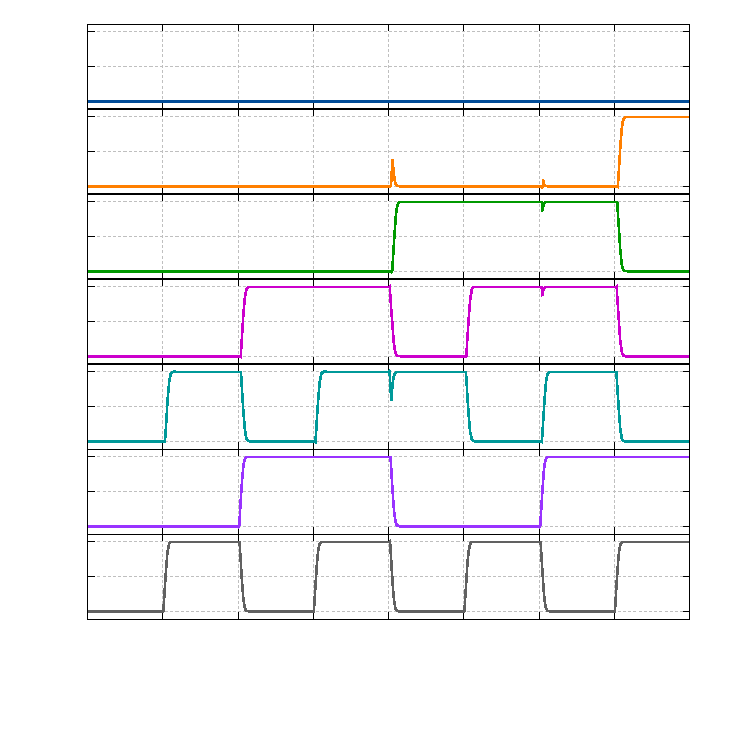
\includegraphics[width={340.10bp},height={340.10bp}]{Immagini/mult-sim}}%
    \gplfronttext
  \end{picture}%
\endgroup

